% Provenance (never printed): old terminale S material on past climates (ice cores,
% pollen, ocean sediments and oxygen isotopes, glacial-interglacial cycles, the
% astronomical rhythm told, climates of deep time), read from data. Owner (Sync 0/1):
% climate archive and proxy, ice core, glacial period, interglacial and glacial cycle,
% pollen analysis, Last Glacial Maximum. Recalled: glacier, ice sheet, ice age (Book 1,
% grade 8); the first look at the ice-core records (Book 1, grade 9); isotopes
% (physics); greenhouse gases (chemistry); the time scale (Book 1, grade 7). The
% delta notation of isotopes is Book 3's: isotope curves are read here as told,
% without a definition. The orbital theory of climate belongs to a university book:
% told here only. Physical science only, in the IPCC's calibrated words.
% Figures: figdata/grade-12/ice_age_records.py (tests/grade-12/test_ice_age_records.py).
\chapter{Lire les climats du passé}\label{ch:g12:past-climates}

Au Dôme~C, à \qty{3233}{m} d'altitude sur la calotte glaciaire de
l'Antarctique de l'Est, l'air est en moyenne à environ
\qty{-55}{\degreeCelsius} sur l'année. Un forage y a été arrêté à
\qty{3260}{m} de profondeur, à environ \qty{15}{m} au-dessus de la roche
située sous la glace. La glace la plus profonde qu'il a remontée renferme
de minuscules bulles d'air vieilles de quelque \num{800000} ans~: un
échantillon de l'atmosphère bien antérieur aux premiers agriculteurs. Ce
chapitre lit le climat du passé dans la glace, dans la boue des lacs et des
fonds océaniques, et dans les roches, et cherche ce qu'il nous dit
d'aujourd'hui.
% ledger: ipev:concordia, edc3:drilling, jouzel07:edc

\begin{omfigure}
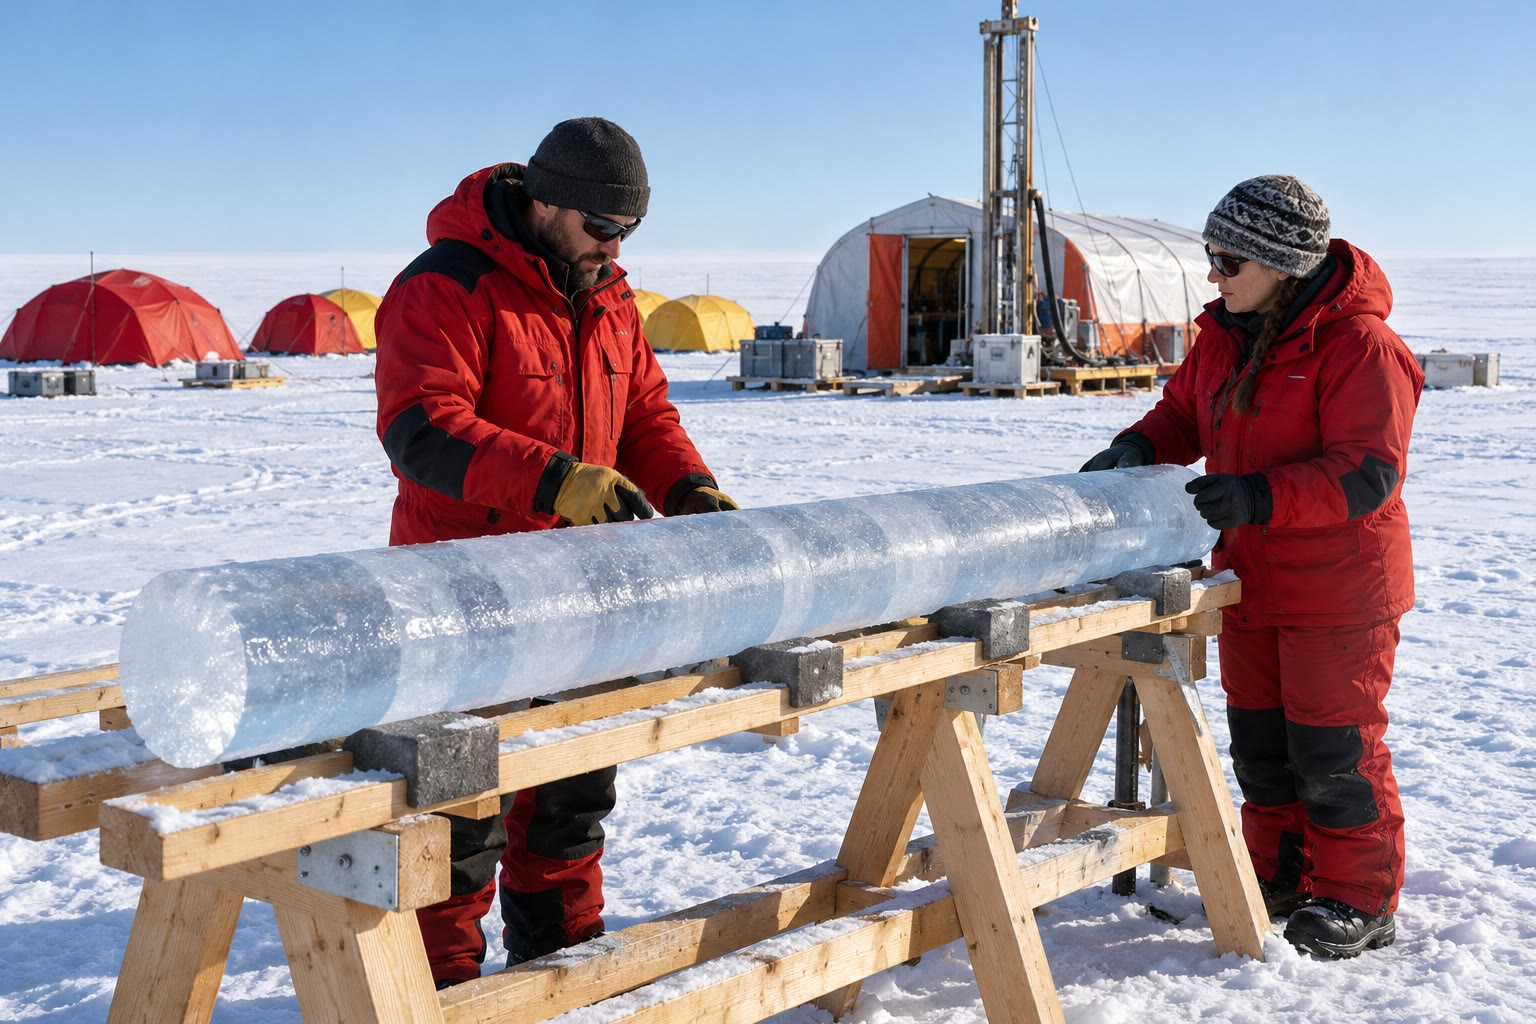
\includegraphics[width=0.56\linewidth]{images/book2/ai/g12-ice-coring-camp.jpg}

{\small Un camp de carottage sur une calotte glaciaire polaire~: le
carottier travaille sous la tour et l'abri, et chaque tronçon de carotte
est disposé, décrit et emballé avant de partir pour le laboratoire.
Illustration générée par IA.}
\end{omfigure}

\begin{recall}
Un glacier est une masse de glace qui persiste d'une année à l'autre et
s'écoule sous son propre poids~; une calotte glaciaire couvre une grande
partie d'un continent~; une glaciation est une longue période froide
pendant laquelle les calottes glaciaires s'étendent bien au-delà des pôles
(livre~1, année~8). Dans les \omterm{def:g12:past-climates:ice-core}{carottes de glace} de l'Antarctique, la neige
enregistre la température de l'air et les bulles gardent l'air lui-même, et
les deux enregistrements montent et descendent ensemble (livre~1,
année~9). Les atomes d'un même élément peuvent différer par leur nombre de
neutrons~: ces isotopes se comportent de la même façon en chimie mais
diffèrent par leur masse (les livres de physique). Le dioxyde de carbone
est un gaz à effet de serre (les livres de chimie). La période quaternaire
a commencé il y a 2.58 millions d'années (livre~1, année~7).
\end{recall}
% ledger: ics:base.Quaternary (shared), nasaeo:o18 (snow poor in heavy isotopes)

\section{Archives et indicateurs}

Personne n'a mesuré la température de l'air il y a \num{20000} ans. Mais la
Terre a tenu des registres sans le vouloir~: couches de glace et de boue,
coquilles et troncs d'arbres, qui ont chacun changé avec le climat dans
lequel ils se sont formés.

\begin{definition}[Archive climatique~; indicateur climatique]\label{def:g12:past-climates:proxy}
Une \emph{archive climatique}\index{archive climatique} est un matériau
naturel déposé en couches successives, qui garde une trace du climat de
l'époque où il s'est formé~: glace polaire, sédiments des lacs et des fonds
océaniques, cernes des arbres, coraux, concrétions des grottes. Un
\emph{indicateur climatique}\index{indicateur climatique} (ou
«~proxy~») est une grandeur mesurée dans une archive, qui tient lieu
d'une variable climatique qui n'a pas été mesurée~: la part d'isotopes
lourds dans la neige ancienne pour la température de l'air, la part de
chaque type de pollen dans la boue d'un lac pour la végétation, et donc
pour le climat.
\end{definition}
% ledger: ncei:proxy, ncei:pollen, nasaeo:o18

\begin{center}
\small
\begin{tabular}{|l|l|l|}
\hline
\textbf{archive} & \textbf{\omterm{def:g12:past-climates:proxy}{indicateur}} & \textbf{renseigne sur} \\
\hline
glace polaire & isotopes lourds de la glace & température de l'air sur la glace \\
 & air des bulles & dioxyde de carbone, méthane \\
sédiments lacustres, tourbe & pollen & végétation, puis climat \\
sédiments océaniques & oxygène 18 des coquilles & volume de glace, température des fonds \\
cernes des arbres & largeur des cernes & conditions de croissance, année par année \\
coraux, concrétions & isotopes, bandes de croissance & température de la mer ou de l'air, pluie \\
\hline
\end{tabular}

\medskip
{\small Les principales \omterm{def:g12:past-climates:proxy}{archives climatiques} et quelques-uns de leurs
\omterm{def:g12:past-climates:proxy}{indicateurs}.}
\end{center}
% ledger: ncei:proxy, nasaeo:o18

Tout \omterm{def:g12:past-climates:proxy}{indicateur} exige deux choses avant de pouvoir être lu. Il lui faut une
\emph{horloge}~: l'âge de chaque couche, obtenu en comptant les couches
annuelles là où on les voit, par datation radiométrique
(\cref{ch:g12:age-of-the-earth}), ou en raccordant l'enregistrement à un
autre déjà daté. Et il lui faut un \emph{étalonnage}~: le lien entre ce que
l'on mesure et la variable climatique, établi aujourd'hui, là où les deux
peuvent être mesurés ensemble.

\begin{method}[Lire un enregistrement d'indicateur]
\begin{enumerate}
  \item Repérer l'archive et l'\omterm{def:g12:past-climates:proxy}{indicateur}~: qu'a-t-on mesuré, et dans
        quoi~?
  \item Repérer dans quel sens le temps s'écoule sur l'axe, et dans quelle
        unité~; vérifier si l'axe de l'\omterm{def:g12:past-climates:proxy}{indicateur} est inversé.
  \item Traduire l'\omterm{def:g12:past-climates:proxy}{indicateur}~: une valeur plus élevée signifie-t-elle plus
        chaud ou plus froid, plus de glace ou moins~?
  \item Noter l'espacement des échantillons~: un enregistrement dont les
        points sont distants de \num{2000} ans ne peut pas montrer un
        changement qui a duré un siècle.
  \item Lire les valeurs aux dates demandées, ou les moyennes sur un
        intervalle, et calculer les variations et les vitesses.
  \item Dire ce que l'enregistrement montre en son site, et seulement
        ensuite s'il vaut pour la Terre entière.
\end{enumerate}
\end{method}

\section{Les carottes de glace}

\begin{definition}[Carotte de glace]\label{def:g12:past-climates:ice-core}
Une \emph{carotte de glace}\index{carotte de glace} est un cylindre de glace
extrait par forage d'une calotte glaciaire ou d'un glacier. Sa profondeur
donne l'âge de la glace, d'autant plus vieille qu'elle est profonde~; la
glace enregistre la température de l'air dans lequel sa neige est tombée,
et ses bulles gardent des échantillons de l'air de l'époque.
\end{definition}
% ledger: ncei:proxy, jouzel07:edc

La neige fraîche est faite surtout d'air. Enfouie sous la neige des années
suivantes, elle est tassée en \emph{névé}, une neige compactée dont les
pores laissent encore passer l'air. À une masse volumique d'environ 820 à
\qty{830}{kg/m^3}, atteinte entre 50 et \qty{120}{m} de profondeur, les
pores se ferment et l'air est enfermé dans des bulles. La glace garde donc
deux enregistrements différents. L'air des bulles est un échantillon de
l'atmosphère, dont on mesure au laboratoire le dioxyde de carbone et le
méthane. La glace elle-même garde la température~: les molécules d'eau qui
contiennent un isotope lourd (le deutérium ou l'oxygène~18) se condensent
plus facilement que les légères~; plus l'air est froid sur le chemin du
pôle, plus la neige s'appauvrit donc en isotopes lourds.
% ledger: firn:close-off, nasaeo:o18

\begin{omfigure}
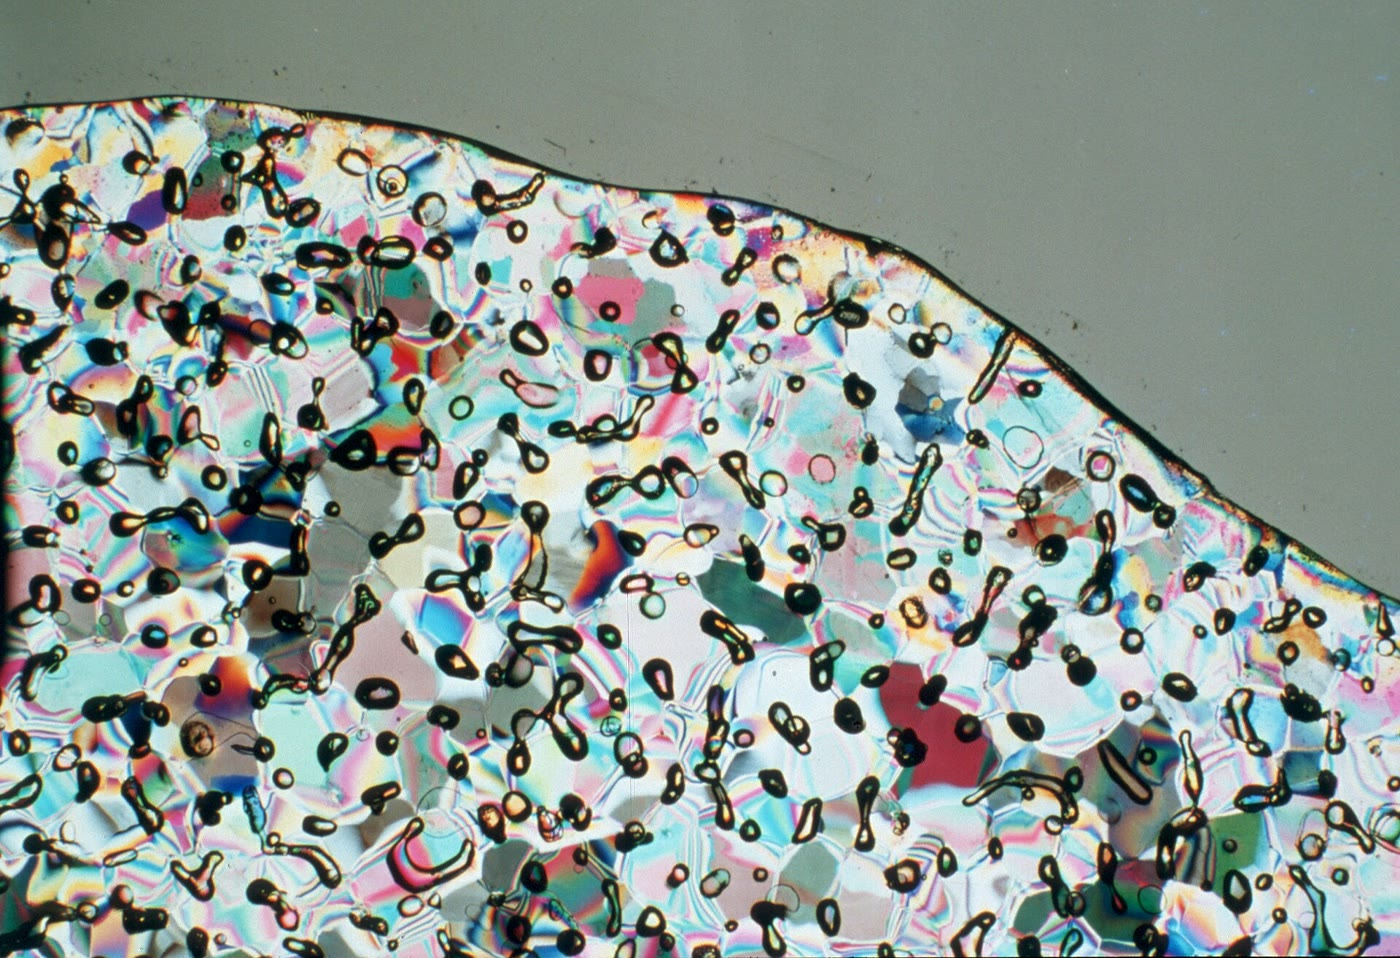
\includegraphics[width=0.50\linewidth]{images/book2/g12-ice-bubbles.jpg}

{\small Une lamelle de glace antarctique vue en lumière polarisée, qui
colore les cristaux de glace~: les points sombres sont des bulles d'air
piégé. Photographie CSIRO Atmospheric Research, CC~BY~3.0 (Wikimedia
Commons).}
\end{omfigure}
% ledger: photo:g12-ice-bubbles

Le deutérium de la carotte du Dôme~C a été converti en une température
au-dessus de la glace, exprimée comme une variation par rapport à la
moyenne des mille dernières années. Le dioxyde de carbone provient des
bulles de plusieurs carottes antarctiques, réunies en un seul
enregistrement. Les deux sont tracés ci-dessous sur un même axe du temps.

\begin{omfigure}
\begin{tikzpicture}
\begin{axis}[omrecord, scale only axis, width=0.74\linewidth, height=4.8cm,
  xmin=0, xmax=800, x dir=reverse, ymin=-12, ymax=8, axis y line*=left,
  xtick={0,100,...,800}, ytick={-10,-5,0,5},
  xlabel={milliers d'années avant 1950},
  ylabel={variation de température (\unit{\degreeCelsius})}]
% data:edc-jouzel, 2-kyr means (figdata/grade-12/ice_age_records.py)
\addplot[omWarm, line width=0.7pt] table[x=age_kyr, y=temp_C] {figdata/out/grade-12-ice_age_records-edc.dat};
\end{axis}
\begin{axis}[scale only axis, width=0.74\linewidth, height=4.8cm,
  xmin=0, xmax=800, x dir=reverse, ymin=60, ymax=320, axis y line*=right,
  axis x line=none, ytick={180,220,260,300}, ylabel={dioxyde de carbone (ppm)},
  every axis label/.append style={font=\small}, tick label style={font=\small}]
% data:co2-bereiter, 2-kyr means
\addplot[black, line width=0.7pt] table[x=age_kyr, y=co2_ppm] {figdata/out/grade-12-ice_age_records-co2.dat};
\coordinate (lt) at (axis cs:560,70);
\coordinate (lc) at (axis cs:560,312);
\end{axis}
\node[font=\scriptsize, text=omWarm, anchor=south] at (lt) {température au Dôme~C (échelle de gauche)};
\node[font=\scriptsize, anchor=north] at (lc) {dioxyde de carbone (échelle de droite)};
\end{tikzpicture}

{\small Huit cent mille ans de glace antarctique, en moyennes par pas de
\num{2000} ans. En rouge~: la température au Dôme~C par rapport aux mille
dernières années (Jouzel et ses collègues, 2007)~; en noir~: le dioxyde de
carbone des bulles (Bereiter et ses collègues, 2015). Le présent est à
droite.}
\end{omfigure}
% ledger: data:edc-jouzel, data:co2-bereiter

Les deux courbes ont un même motif~: une lente glissade irrégulière vers le
froid sur des dizaines de milliers d'années, puis une remontée rapide vers
la chaleur, puis de nouveau la glissade.

\begin{definition}[Période glaciaire~; interglaciaire~; cycle glaciaire]\label{def:g12:past-climates:glacial-cycle}
Une \emph{période glaciaire}\index{periode glaciaire@période glaciaire} est
un intervalle froid au sein d'une glaciation, pendant lequel les calottes
glaciaires s'étendent bien au-delà de leur taille actuelle. Un
\emph{interglaciaire}\index{interglaciaire} est un intervalle chaud entre
deux périodes glaciaires, avec des calottes glaciaires proches de celles
d'aujourd'hui ou plus petites~; nous vivons dans l'un d'eux, qui a commencé
il y a environ \num{11000} ans. Un \emph{cycle
glaciaire}\index{cycle glaciaire} est une période glaciaire suivie de
l'interglaciaire qui la termine.
\end{definition}
% ledger: ipcc:ref-periods (LDT ends 11 ka); the count of cycles is read from the figure (data:edc-jouzel)

Sur l'ensemble de l'enregistrement, la température au Dôme~C varie de
\qty{-10.6}{\degreeCelsius}, il y a environ \num{24000} ans, à
\qty{+5.5}{\degreeCelsius}, il y a environ \num{129000} ans~; le dioxyde
de carbone, de \qty{174}{ppm} à \qty{299}{ppm}. La figure, moyennée sur
\num{2000} ans, adoucit un peu ces extrêmes. En comptant les pics chauds,
on trouve huit ou neuf \omterm{def:g12:past-climates:glacial-cycle}{cycles glaciaires}, et le rythme le plus fort de
l'enregistrement de température, calculé à partir de ses données, a une
période d'environ \num{98000} ans.
% ledger: data:edc-jouzel, data:co2-bereiter (ice_age_records.py: edc_min_C -10.58 at 24.0 kyr, edc_max_C 5.46 at 128.7 kyr, co2 173.71 and 298.6, edc_period_kyr 97.5)

\begin{proposition}[Température et dioxyde de carbone varient ensemble]\label{prop:g12:past-climates:correlation}
% ledger: data:edc-jouzel, data:co2-bereiter (ice_age_records.py: r_temp_co2 0.9165, fit 266.57 + 7.827 T, 1639 pairs)
Au cours des \num{800000} dernières années, la température antarctique et
le dioxyde de carbone de l'air ont varié ensemble. Associer chacune des
1639 mesures de dioxyde de carbone de plus de \num{2000} ans à la
température du Dôme~C au même âge donne un coefficient de corrélation
$r = 0.92$, et la droite des moindres carrés
\[
  \mathrm{CO_2} \approx \qty{267}{ppm} + \qty{7.8}{ppm/\degreeCelsius} \times \Delta T ,
\]
où $\Delta T$ est la variation de température au Dôme~C.
\end{proposition}

\begin{proof}[Comment on le calcule]
Pour chaque échantillon de dioxyde de carbone, on lit la température à son
âge dans l'enregistrement du Dôme~C, par interpolation entre les deux
points de température les plus proches. Le coefficient de corrélation des
1639 couples, un nombre compris entre $-1$ et $1$ qui mesure à quel point
les points sont proches d'une droite (les livres de mathématiques), se
calcule avec la droite des moindres carrés~; les deux sont calculés dans le
script de la figure et vérifiés par son test.
\end{proof}

\begin{omfigure}
\begin{tikzpicture}
\begin{axis}[omrecord, width=0.70\linewidth, height=5.2cm, xmin=-12, xmax=6,
  ymin=160, ymax=310, xlabel={variation de température au Dôme~C (\unit{\degreeCelsius})},
  ylabel={dioxyde de carbone (ppm)}]
% data:edc-jouzel, data:co2-bereiter (pairs and fit in ice_age_records.py)
\addplot[only marks, mark=*, mark size=0.6pt, omDef, opacity=0.45] table[x=temp_C, y=co2_ppm] {figdata/out/grade-12-ice_age_records-pairs.dat};
\addplot[omThm, line width=1pt] table[x=temp_C, y=co2_ppm] {figdata/out/grade-12-ice_age_records-fit.dat};
\node[font=\scriptsize, text=omThm, anchor=south east, fill=white, inner sep=1pt] at (axis cs:-1.5,295) {droite des moindres carrés, $r = 0.92$};
\end{axis}
\end{tikzpicture}

{\small Chaque point est une mesure de dioxyde de carbone de la glace
antarctique, placée à la température du Dôme~C du même âge~: les époques
froides avaient peu de dioxyde de carbone, les époques chaudes beaucoup
plus. Calculé d'après Jouzel et ses collègues (2007) et Bereiter et ses
collègues (2015).}
\end{omfigure}

Une corrélation ne dit ni lequel a changé le premier, ni si une troisième
cause a fait varier les deux~: le coefficient serait le même si la
température pilotait le dioxyde de carbone, si le dioxyde de carbone
pilotait la température, ou si chacun poussait l'autre. Ce qui fixe le
rythme d'environ \num{100000} ans est raconté dans la section sur l'océan,
plus loin, et la façon dont le dioxyde de carbone agit sur la température
au \cref{ch:g12:climate-change}.

\subsection{Le dernier maximum glaciaire}

\begin{definition}[Dernier maximum glaciaire]\label{def:g12:past-climates:lgm}
Le \emph{dernier maximum glaciaire}\index{dernier maximum glaciaire} est
l'époque, il y a environ \num{23000} à \num{19000} ans, où les calottes
glaciaires de la dernière \omterm{def:g12:past-climates:glacial-cycle}{période glaciaire} atteignaient leur plus grande
extension.
\end{definition}
% ledger: ipcc:ref-periods

Au \omterm{def:g12:past-climates:lgm}{dernier maximum glaciaire}, des calottes glaciaires couvraient une grande
partie de l'Amérique du Nord et du nord-ouest de l'Eurasie, et le climat
était plus sec et plus poussiéreux qu'aujourd'hui. Les évaluations
estiment que la température moyenne à la surface du globe était inférieure
de \qty{5}{\degreeCelsius} à \qty{7}{\degreeCelsius} à celle de 1850--1900
(\emph{degré de confiance moyen}), avec un dioxyde de carbone de 188 à
\qty{194}{ppm}. L'eau stockée dans les calottes glaciaires venait de
l'océan~: le niveau moyen de la mer se trouvait 125 à \qty{134}{m}
au-dessous du niveau actuel.
% ledger: ipcc:ref-periods, ipcc:lgm-cooling, ipcc:fig2-34, ipcc:lgm-sea, lambeck14:lgm

Une mer plus basse découvre les fonds peu profonds qui entourent les
continents. La carte ci-dessous abaisse la mer de \qty{130}{m}, le milieu
de cet intervalle, sur les fonds actuels de l'Asie du Sud-Est.

\begin{omfigure}
\begin{tikzpicture}
\begin{axis}[omrecord, axis equal image, width=0.62\linewidth, xmin=92, xmax=122,
  ymin=-11, ymax=24, grid=none, axis x line=box, axis y line=box,
  xtick={95,105,115}, ytick={-10,-5,...,20},
  xticklabel={\pgfmathprintnumber{\tick}\textdegree E},
  yticklabels={10\textdegree S, 5\textdegree S, 0\textdegree, 5\textdegree N, 10\textdegree N, 15\textdegree N, 20\textdegree N}]
% data:b2-etopo-sunda (raster computed in ice_age_records.py; sea level lowered by 130 m)
\addplot graphics[xmin=91.95, xmax=122.05, ymin=-11.05, ymax=24.05] {figdata/out/grade-12-ice_age_records-sunda.png};
\node[font=\scriptsize] at (axis cs:114.5,0.5) {Bornéo};
\node[font=\scriptsize, rotate=-45] at (axis cs:101.9,-1.3) {Sumatra};
\node[font=\scriptsize] at (axis cs:110.5,-8.6) {Java};
\node[font=\scriptsize, rotate=-60] at (axis cs:102.2,4.0) {pén. Malaise};
\node[font=\scriptsize] at (axis cs:103,16.5) {Indochine};
\node[font=\scriptsize, align=center] at (axis cs:106.5,3.5) {plateau\\de la Sonde};
\node[font=\scriptsize, align=center] at (axis cs:114.5,13) {mer de Chine\\méridionale};
\node[font=\scriptsize, align=center] at (axis cs:96,-6) {océan\\Indien};
\end{axis}
\end{tikzpicture}

{\small L'Asie du Sud-Est avec une mer plus basse de \qty{130}{m}
qu'aujourd'hui. En vert~: les terres actuelles~; en beige~: les fonds
qu'un niveau de la mer plus bas de \qty{130}{m} découvre~; en bleu~: la
mer. Le relief actuel est utilisé~: le tracé des côtes n'est donc
qu'approximatif. Calculé d'après le relief ETOPO1 (NOAA), tous les
0.1~degré.}
\end{omfigure}
% ledger: data:b2-etopo-sunda, ipcc:lgm-sea

Bornéo, Sumatra et Java ne forment plus qu'une seule terre avec la
péninsule Malaise et l'Indochine~: le plateau de la Sonde, aujourd'hui sous
une mer peu profonde, était émergé. Sur la carte, une baisse d'environ
\qty{36}{m} seulement suffit à relier Bornéo à l'Asie, et Sumatra et Java
s'y relient plus tôt. Sur la carte, les terres émergées passent de 4.11 à
7.16 millions de kilomètres carrés, soit 1.74 fois plus. Sur la Terre
entière, la même baisse de \qty{130}{m} fait passer la part de la surface
émergée de \qty{29.0}{\percent} à \qty{33.5}{\percent}, soit environ 23
millions de kilomètres carrés de terres nouvelles.
% ledger: data:b2-etopo-sunda, data:etopo1 (ice_age_records.py: borneo_link_m -36; sunda_land_now_km2 4.105e6, lgm 7.161e6, ratio 1.744; world_land_now_frac 0.2904, lgm 0.3352, world_gain_km2 2.285e7)

\begin{example}[La dernière déglaciation]
Le réchauffement qui a suivi le \omterm{def:g12:past-climates:lgm}{dernier maximum glaciaire} s'appelle la
dernière transition déglaciaire~; les évaluations la placent entre il y a
environ \num{18000} et \num{11000} ans. Dans l'enregistrement du Dôme~C,
la température moyenne du \omterm{def:g12:past-climates:lgm}{dernier maximum glaciaire} (il y a \num{23000} à
\num{19000} ans) est de \qty{-9.4}{\degreeCelsius}~; la moyenne de
l'intervalle suivant, il y a \num{11000} à \num{9000} ans, est de
\qty{-0.4}{\degreeCelsius}. L'air au-dessus de l'Antarctique s'est
réchauffé de \qty{9.0}{\degreeCelsius}, tandis que son dioxyde de carbone
passait de \qty{190}{ppm} à \qty{264}{ppm}, soit \qty{74}{ppm} de plus. Sur
la Terre entière, le réchauffement a été égal au refroidissement évalué de
5 à \qty{7}{\degreeCelsius}, environ \qty{6}{\degreeCelsius}, réparti sur
les \num{7000} ans de la transition~:
\[
  \frac{\qty{6}{\degreeCelsius}}{\num{7000}\ \text{ans}} \approx
  \qty{0.86}{\degreeCelsius} \text{ par millier d'années.}
\]
Pendant ce temps, le niveau de la mer est passé d'environ \qty{-120}{m} à
\qty{-50}{m}, soit environ \qty{10}{mm} par an en moyenne.
\end{example}
% ledger: ipcc:ref-periods, ipcc:lgm-cooling, ipcc:lgm-sea, data:edc-jouzel, data:co2-bereiter (ice_age_records.py: edc_lgm_C -9.389, edc_holo_C -0.360, rise 9.029; co2 189.67, 264.10, rise 74.43; ldt_mean_rate 0.857)

\begin{omfigure}
\begin{tikzpicture}
\begin{axis}[omrecord, scale only axis, width=0.74\linewidth, height=4.6cm,
  xmin=0, xmax=30, x dir=reverse, ymin=-11, ymax=12, axis y line*=left,
  xtick={0,5,...,30}, ytick={-10,-5,0},
  xlabel={milliers d'années avant 1950},
  ylabel={variation de température (\unit{\degreeCelsius})}]
\fill[omDef!10] (axis cs:23,-11) rectangle (axis cs:19,12);
\fill[omProp!12] (axis cs:18,-11) rectangle (axis cs:11,12);
% data:edc-jouzel, every sample
\addplot[omWarm, line width=0.6pt] table[x=age_kyr, y=temp_C] {figdata/out/grade-12-ice_age_records-edc30.dat};
\coordinate (lgm) at (axis cs:21,11.6);
\coordinate (ldt) at (axis cs:14.5,11.6);
\coordinate (lt) at (axis cs:5.5,-3.6);
\end{axis}
\begin{axis}[scale only axis, width=0.74\linewidth, height=4.6cm,
  xmin=0, xmax=30, x dir=reverse, ymin=60, ymax=290, axis y line*=right,
  axis x line=none, ytick={200,240,280}, ylabel={dioxyde de carbone (ppm)},
  every axis label/.append style={font=\small}, tick label style={font=\small}]
% data:co2-bereiter, every sample
\addplot[black, line width=0.6pt, mark=*, mark size=0.5pt] table[x=age_kyr, y=co2_ppm] {figdata/out/grade-12-ice_age_records-co230.dat};
\coordinate (lc) at (axis cs:26.5,196);
\end{axis}
\node[font=\scriptsize, anchor=north, align=center] at (lgm) {dernier maximum\\glaciaire};
\node[font=\scriptsize, anchor=north, align=center] at (ldt) {dernière transition\\déglaciaire};
\node[font=\scriptsize, text=omWarm, anchor=north] at (lt) {température (gauche)};
\node[font=\scriptsize, anchor=south] at (lc) {dioxyde de carbone (droite)};
\end{tikzpicture}

{\small Les \num{30000} dernières années au Dôme~C, toutes les mesures~:
la température (en rouge) et le dioxyde de carbone (en noir) remontent
ensemble au sortir du \omterm{def:g12:past-climates:lgm}{dernier maximum glaciaire}. En grisé~: le \omterm{def:g12:past-climates:lgm}{dernier
maximum glaciaire} et la dernière transition déglaciaire, tels que les date
le GIEC. Données~: Jouzel et ses collègues (2007), Bereiter et ses
collègues (2015).}
\end{omfigure}
% ledger: data:edc-jouzel, data:co2-bereiter, ipcc:ref-periods

\section{Le pollen}

Chaque printemps, les plantes libèrent des nuages de pollen. L'essentiel
se perd, mais une partie tombe sur les lacs et les tourbières, coule et
s'enfouit dans la boue, où elle garde la trace de la végétation qui
poussait alentour. Et les grains de chaque type de plante ont leur propre
forme et leur propre taille.
% ledger: ncei:pollen

\begin{omfigure}
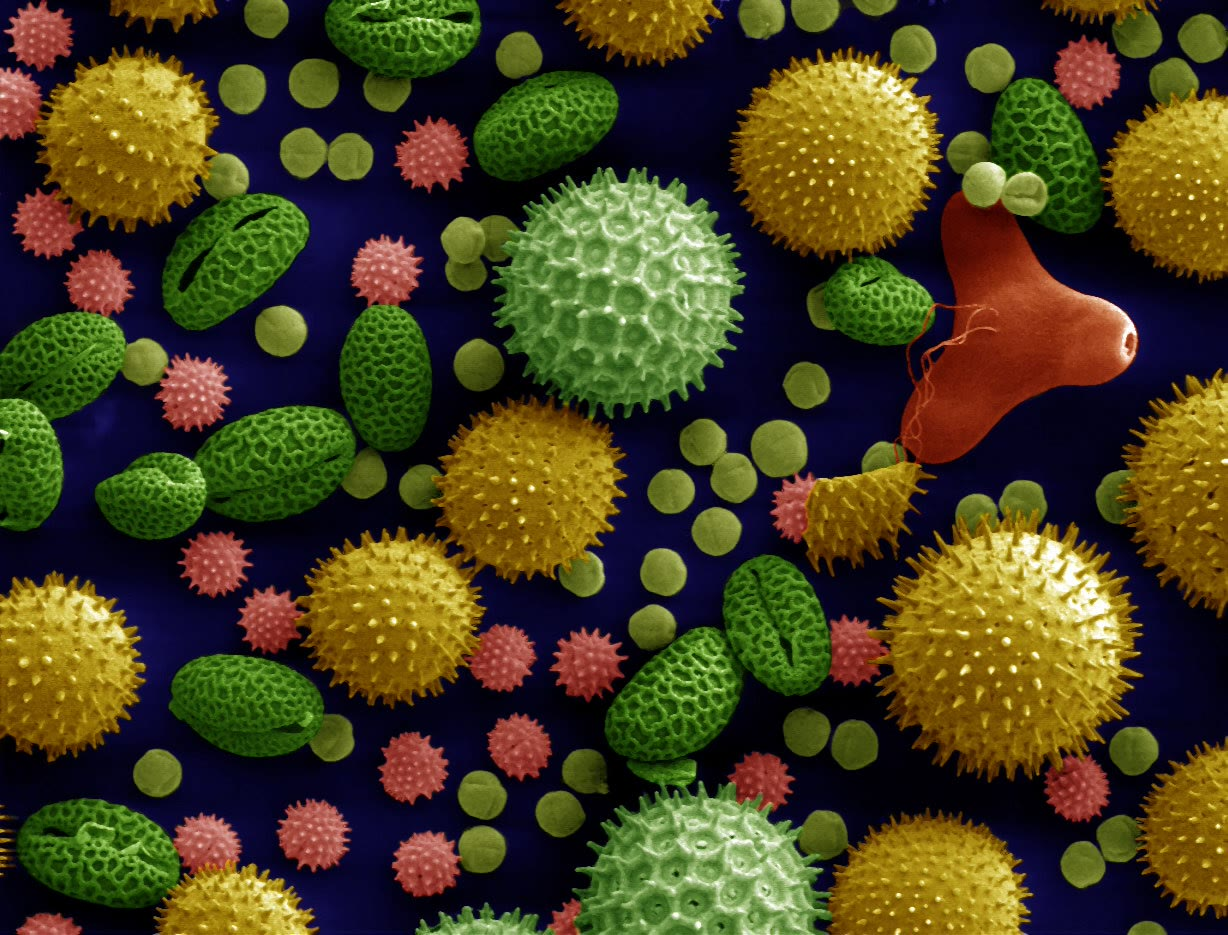
\includegraphics[width=0.46\linewidth]{images/book2/g12-pollen-sem.jpg}

{\small Grains de pollen de cinq plantes communes (tournesol, ipomée,
rose trémière, lis et primevère) vus au microscope électronique à balayage,
en fausses couleurs. Chaque type de plante a sa propre forme de grain.
Dartmouth Electron Microscope Facility (domaine public, via Wikimedia
Commons).}
\end{omfigure}
% ledger: photo:g12-pollen

\begin{definition}[Analyse pollinique]\label{def:g12:past-climates:pollen}
L'\emph{analyse pollinique}\index{analyse pollinique} est la lecture de la
végétation passée à partir du pollen conservé dans les sédiments~: dans
chaque couche d'une carotte, on identifie et on compte les grains, et la
part de chaque type de plante, en pourcentage des grains comptés, est
portée en fonction de la profondeur dans un \emph{diagramme
pollinique}\index{diagramme pollinique}.
\end{definition}
% ledger: ncei:pollen

Le comptage du pollen de cette façon a commencé avec le géologue suédois
Lennart von Post, qui présenta en 1916 le premier \omterm{def:g12:past-climates:pollen}{diagramme pollinique}
moderne, chiffré~; un tel diagramme montre la profondeur vers le bas de la
page, et une courbe pour chaque type de plante. La végétation, à son tour,
renseigne sur le climat~: des graminées et d'autres herbacées presque sans
arbres signalent un paysage ouvert et froid, tandis que le chêne et le
noisetier ont besoin d'étés chauds.
% ledger: rull18:von-post; the Varden diagram is invented (ice_age_records.py POLLEN)

\begin{omfigure}
\begin{tikzpicture}
\pgfplotsset{pollen/.style={scale only axis, height=6cm, ymin=300, ymax=600,
  y dir=reverse, xmin=0, axis x line*=bottom, axis y line*=left, axis line style={-},
  tick label style={font=\scriptsize}, title style={font=\small, yshift=-4pt, text depth=0.25ex, text height=1.6ex},
  ytick={300,350,...,600}, xmajorgrids, ymajorgrids,
  grid style={gray!22, line width=0.3pt}}}
\begin{axis}[pollen, name=p1, width=3.0cm, xmax=100, xtick={0,20,...,80}, title={herbacées},
  ylabel={profondeur (cm)}, every axis label/.append style={font=\small}]
\addplot[fill=omLithSand, draw=black!70, line width=0.4pt] table[x=pct, y=depth_cm] {figdata/out/grade-12-ice_age_records-pol-herbs.dat};
\coordinate (z1) at (axis cs:0,550);
\coordinate (z2) at (axis cs:0,470);
\coordinate (z3) at (axis cs:0,425);
\end{axis}
\begin{axis}[pollen, name=p2, at={(p1.south east)}, anchor=south west, xshift=0.3cm,
  width=1.8cm, xmax=60, xtick={0,20,40}, title={bouleau}, yticklabels={}]
\addplot[fill=omHypsLandB, draw=black!70, line width=0.4pt] table[x=pct, y=depth_cm] {figdata/out/grade-12-ice_age_records-pol-birch.dat};
\end{axis}
\begin{axis}[pollen, name=p3, at={(p2.south east)}, anchor=south west, xshift=0.3cm,
  width=1.8cm, xmax=60, xtick={0,20,40}, title={pin}, yticklabels={}]
\addplot[fill=omHypsLandA, draw=black!70, line width=0.4pt] table[x=pct, y=depth_cm] {figdata/out/grade-12-ice_age_records-pol-pine.dat};
\end{axis}
\begin{axis}[pollen, name=p4, at={(p3.south east)}, anchor=south west, xshift=0.3cm,
  width=1.2cm, xmax=40, xtick={0,20}, title={noisetier}, yticklabels={}]
\addplot[fill=omHypsLandD, draw=black!70, line width=0.4pt] table[x=pct, y=depth_cm] {figdata/out/grade-12-ice_age_records-pol-hazel.dat};
\end{axis}
\begin{axis}[pollen, name=p5, at={(p4.south east)}, anchor=south west, xshift=0.3cm,
  width=1.5cm, xmax=50, xtick={0,20,40}, title={chêne}, yticklabels={}]
\addplot[fill=omHypsLandE, draw=black!70, line width=0.4pt] table[x=pct, y=depth_cm] {figdata/out/grade-12-ice_age_records-pol-oak.dat};
\coordinate (e1) at (axis cs:50,550);
\coordinate (e2) at (axis cs:50,470);
\coordinate (e3) at (axis cs:50,425);
\coordinate (top) at (axis cs:50,300);
\coordinate (bot) at (axis cs:50,600);
\end{axis}
\draw[densely dashed, black!70] (z1) -- (e1 -| p5.east);
\draw[densely dashed, black!70] (z2) -- (e2 -| p5.east);
\draw[densely dashed, black!70] (z3) -- (e3 -| p5.east);
\node[font=\scriptsize, anchor=west] at ($(bot -| p5.east)!0.5!(e1 -| p5.east)$) {zone 1};
\node[font=\scriptsize, anchor=west] at ($(e1 -| p5.east)!0.5!(e2 -| p5.east)$) {zone 2};
\node[font=\scriptsize, anchor=west] at ($(e2 -| p5.east)!0.5!(e3 -| p5.east)$) {zone 3};
\node[font=\scriptsize, anchor=west] at ($(e3 -| p5.east)!0.5!(top -| p5.east)$) {zone 4};
\node[font=\scriptsize, anchor=north] at ($(p1.south)!0.5!(p5.south)+(0,-0.45)$) {pourcentage du pollen compté};
\end{tikzpicture}

{\small Un \omterm{def:g12:past-climates:pollen}{diagramme pollinique} d'un lac des collines de Varden, la région
imaginaire de cette série~: données d'exercice inventées, avec la
succession que l'on observe dans de nombreux lacs de la zone tempérée
fraîche. Le fond de la carotte (\qty{600}{cm}) a \num{14000} ans, le
sommet représenté (\qty{300}{cm}) \num{6000} ans, avec une vitesse de dépôt
constante entre les deux.}
\end{omfigure}
% invented exercise data (ice_age_records.py POLLEN); no ledger row

\begin{method}[Lire un diagramme pollinique]
\begin{enumerate}
  \item Lire l'axe vertical~: la profondeur, les couches les plus anciennes
        en bas~; convertir les profondeurs en âges grâce aux datations de
        la carotte.
  \item Pour chaque couche, repérer les plantes dont les parts sont les
        plus grandes.
  \item Découper la carotte en zones, chacune avec son propre ensemble de
        plantes dominantes~; placer les limites là où les courbes changent
        le plus vite.
  \item Nommer la végétation de chaque zone (herbacées ouvertes, boulaie,
        forêt de pins, forêt de feuillus) et le climat qu'elle exige.
  \item Lire les zones de bas en haut comme une histoire du paysage.
\end{enumerate}
\end{method}

Dans le diagramme ci-dessus, la zone 1 est un paysage d'herbacées, avec
quelques bouleaux~: le pays ouvert et froid laissé par la glace. Dans la
zone 2, le bouleau, arbre robuste, s'étend le premier~; le pin suit dans la
zone 3~; et dans la zone 4, le noisetier et le chêne, qui ont besoin d'étés
chauds, prennent le dessus. Lue de bas en haut, la carotte raconte la fin
de la \omterm{def:g12:past-climates:glacial-cycle}{période glaciaire} et l'arrivée de la chaleur de l'\omterm{def:g12:past-climates:glacial-cycle}{interglaciaire}, à
mesure que la forêt reconquérait le pays.

\section{Les sédiments océaniques et le rythme astronomique}

Sur le fond de l'océan ouvert, la boue s'accumule lentement et sans
interruption, couche après couche, pendant des millions d'années. Elle est
pleine de coquilles de foraminifères~: des organismes unicellulaires dont
la coquille, d'une fraction de millimètre, est souvent en calcite.
Certains flottent près de la surface~; d'autres vivent sur le fond marin.
% ledger: ucmp:forams, lr04:stack (benthic), photo:g12-forams (planktic)

\begin{omfigure}
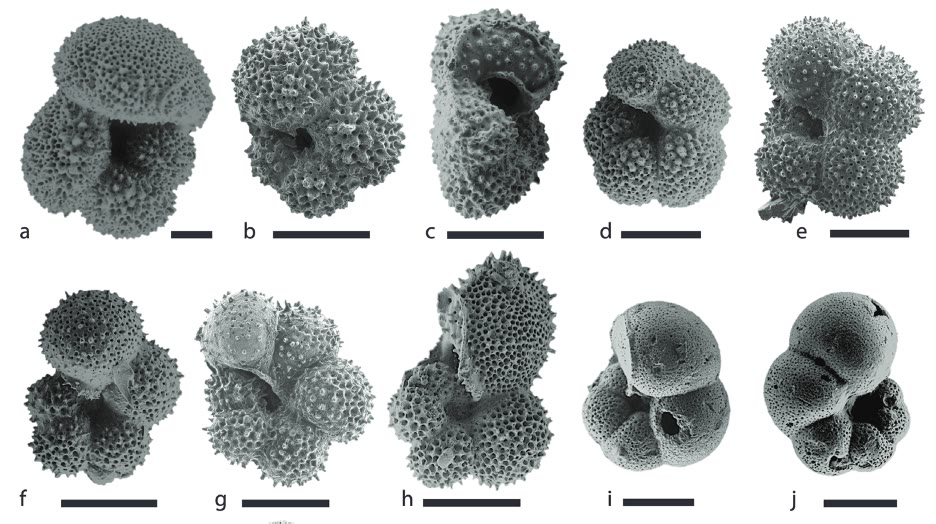
\includegraphics[width=0.62\linewidth]{images/book2/g12-planktic-foraminifera.jpg}

{\small Coquilles de dix espèces de foraminifères qui vivaient en flottant
dans l'océan, vues au microscope électronique à balayage~; chaque barre
d'échelle mesure \qty{150}{\micro\metre}~: chaque coquille a donc à peu
près la taille d'un grain de sable. Marci Robinson, USGS (domaine public,
via Wikimedia Commons).}
\end{omfigure}
% ledger: photo:g12-forams

L'oxygène d'une coquille provient de l'eau de mer. L'eau formée avec
l'isotope léger, l'oxygène~16, s'évapore plus facilement, et la neige qui
construit les calottes glaciaires est donc pauvre en oxygène~18. Quand les
calottes grandissent, elles stockent cette eau légère, et l'océan qui reste
s'enrichit en oxygène~18~; de même pour les coquilles qui y croissent,
d'autant plus que l'eau est froide. La part d'oxygène~18 dans les coquilles
des foraminifères du fond marin, notée
$\delta^{18}\mathrm{O}$ et exprimée en pour mille, est ainsi un \omterm{def:g12:past-climates:proxy}{indicateur}
du volume de glace sur les continents et de la température de l'\omterm{def:g10:layered-ocean:thermocline}{océan
profond}~: plus elle est élevée, plus il y a de glace et plus l'eau est
froide.
% ledger: nasaeo:o18, lr04:stack

L'enregistrement ci-dessous, appelé LR04, empile les mesures de 57 carottes
de tous les océans en une seule courbe de 5.3 millions d'années.

\begin{omfigure}
\begin{tikzpicture}
\begin{axis}[omrecord, scale only axis, width=0.86\linewidth, height=4.8cm,
  xmin=0, xmax=5.32, x dir=reverse, ymin=2.4, ymax=5.3, y dir=reverse,
  xtick={0,0.5,...,5}, ytick={2.5,3,...,5},
  x tick label style={/pgf/number format/.cd, fixed, precision=1},
  y tick label style={/pgf/number format/.cd, fixed, fixed zerofill, precision=1},
  xlabel={millions d'années avant 1950},
  ylabel={$\delta^{18}\mathrm{O}$ des coquilles (\unit{\permil})}]
\fill[omProp!14] (axis cs:1.25,2.4) rectangle (axis cs:0.7,5.3);
% data:lr04 (the stack only; ice_age_records.py)
\addplot[omDef!85!black, line width=0.35pt] table[x=age_Ma, y=d18O] {figdata/out/grade-12-ice_age_records-lr04.dat};
\addplot[omThm, line width=1pt, densely dashed, unbounded coords=jump] table[x=age_Ma, y=d18O] {figdata/out/grade-12-ice_age_records-lr04mean.dat};
\coordinate (mpt) at (axis cs:0.975,2.45);
\coordinate (mm) at (axis cs:5.22,4.92);
\coordinate (arr) at (axis cs:5.12,3.9);
\end{axis}
\node[font=\scriptsize, anchor=north, align=center] at (mpt) {41 000 à\\100 000 ans};
\draw[omThm, line width=1pt, densely dashed] (mm) -- ($(mm)+(0.5,0)$) node[right, font=\scriptsize, text=omThm] {moyennes de 5.3 à 3 et de 1 à 0 million d'années};
\draw[-{Stealth}, black!70] (arr) -- ++(0,-0.9) node[midway, right, font=\scriptsize, align=left] {plus de glace,\\plus froid};
\end{tikzpicture}

{\small Cinq millions d'années de l'\omterm{def:g10:layered-ocean:thermocline}{océan profond} dans les coquilles des
foraminifères du fond marin~; l'axe vertical est inversé, pour que les
époques froides et englacées soient en bas. Les tirets sont les moyennes
de la première et de la dernière partie. En grisé~: le passage d'un rythme
de \num{41000} ans à un rythme d'environ \num{100000} ans. Données~:
Lisiecki et Raymo (2005), l'empilement LR04.}
\end{omfigure}
% ledger: data:lr04, lr04:stack, clark06:mpt

Lu avec la méthode ci-dessus, l'enregistrement dit trois choses.
\begin{itemize}
  \item \emph{La Terre s'est refroidie et sa glace a augmenté.} La valeur
        moyenne passe de \qty{3.03}{\permil} entre 5.3 et 3 millions
        d'années à \qty{4.15}{\permil} sur le dernier million d'années.
  \item \emph{Les oscillations se sont amplifiées.} Les époques glaciaires
        et \omterm{def:g12:past-climates:glacial-cycle}{interglaciaires} alternent tout au long de l'enregistrement, mais
        leurs écarts sont de plus en plus grands~: au \omterm{def:g12:past-climates:lgm}{dernier maximum
        glaciaire}, la valeur était de \qty{4.92}{\permil}, contre
        \qty{3.23}{\permil} aujourd'hui.
  \item \emph{Le rythme a changé.} Entre il y a 2.6 et 1.3 millions d'années, la
        période la plus forte de l'enregistrement, calculée à partir de ses
        données, est de \num{41000} ans~; sur les \num{700000} dernières
        années, elle est d'environ \num{98000} ans, le rythme des \omterm{def:g12:past-climates:ice-core}{carottes
        de glace}. Le changement s'est produit entre il y a environ 1.25 et
        0.7 million d'années.
\end{itemize}
% ledger: data:lr04, clark06:mpt (ice_age_records.py: lr04_mean_3_5Ma 3.032, lr04_mean_0_1Ma 4.147, lr04_lgm 4.92, lr04_today 3.23, periods 41.0 and 98.5 kyr)

Ces périodes ne doivent rien au hasard. En 1976, James Hays, John Imbrie et
Nicholas Shackleton trouvèrent dans les sédiments des océans australs trois
rythmes, de \num{23000}, \num{42000} et environ \num{100000} ans, qui sont
les périodes de lentes variations de l'orbite et de l'axe de la Terre~: la
précession de l'axe, l'inclinaison de l'axe (environ \num{41000} ans) et
la forme de l'orbite (environ \num{100000} ans). Ces variations modifient
la lumière solaire que reçoit chaque latitude à chaque saison, et elles
règlent la cadence des \omterm{def:g12:past-climates:glacial-cycle}{cycles glaciaires}. Comment elles le font, et
pourquoi le lent rythme de \num{100000} ans a pris le dessus, relève d'un
cours universitaire.
% ledger: hays76:periods, nasa:milankovitch, lr04:stack, clark06:mpt

\begin{dated}{2025}
En janvier 2025, le projet Beyond EPICA a annoncé qu'une carotte forée à
Little Dome~C, à environ \qty{35}{km} de la station Concordia, sur le
Dôme~C, contient un enregistrement continu remontant à environ 1.2 million
d'années dans ses \qty{2480}{m} supérieurs. Il couvre l'époque où le rythme
glaciaire est passé de \num{41000} à \num{100000} ans~; la glace et son air
sont en cours d'analyse.
\end{dated}
% ledger: ku25:beyond-epica, ipev25:little-dome-c

\section{Les climats des temps géologiques}

Au-delà des \omterm{def:g12:past-climates:ice-core}{carottes de glace}, les climats du passé se lisent dans les
sédiments, les feuilles et les sols fossiles, et les isotopes. Le GIEC a
retenu quelques \emph{périodes de référence}, bien étudiées, dont les
climats aident à juger les changements d'aujourd'hui et de demain. Le
graphique ci-dessous donne leur température moyenne à la surface du globe,
par rapport à 1850--1900.

\begin{omfigure}
\begin{tikzpicture}
\begin{axis}[omrecord, width=0.86\linewidth, height=5.4cm, xmin=-9, xmax=27,
  ymin=0.4, ymax=6.6, y dir=reverse, ytick={1,...,6}, ymajorgrids=false,
  yticklabels={{PETM, 56 Ma}, {EECO, 53--49 Ma}, {MPWP, 3.3--3.0 Ma},
    {LIG, 129--116 ka}, {LGM, 23--19 ka}, {MH, 6.5--5.5 ka}},
  y tick label style={font=\scriptsize},
  xlabel={température par rapport à 1850--1900 (\unit{\degreeCelsius})}]
% ipcc:fig2-34 (DEEP in ice_age_records.py)
\addplot[draw=none, mark=none, restrict expr to domain={\thisrow{tlo}}{0:30},
  error bars/.cd, x dir=both, x explicit,
  error bar style={line width=5pt, omWarm!75}, error mark=none]
  table[x expr={(\thisrow{tlo}+\thisrow{thi})/2}, y=idx,
        x error expr={(\thisrow{thi}-\thisrow{tlo})/2}] {figdata/out/grade-12-ice_age_records-deep.dat};
\addplot[draw=none, mark=none, restrict expr to domain={\thisrow{tlo}}{-30:-0.01},
  error bars/.cd, x dir=both, x explicit,
  error bar style={line width=5pt, omCold!75}, error mark=none]
  table[x expr={(\thisrow{tlo}+\thisrow{thi})/2}, y=idx,
        x error expr={(\thisrow{thi}-\thisrow{tlo})/2}] {figdata/out/grade-12-ice_age_records-deep.dat};
\draw[black!60] (axis cs:0,0.4) -- (axis cs:0,6.6);
\draw[omThm, densely dashed, line width=0.8pt] (axis cs:1.09,0.4) -- (axis cs:1.09,6.6);
\node[font=\scriptsize, text=omThm, anchor=west, fill=white, inner sep=1pt] at (axis cs:1.6,4.55) {2011--2020};
\end{axis}
\end{tikzpicture}

{\small Température moyenne à la surface du globe de six périodes de
référence du passé, fourchettes très probables, par rapport à 1850--1900~;
en tirets~: la décennie 2011--2020. Sigles anglais~: PETM, maximum
thermique du Paléocène--Éocène~; EECO, optimum climatique de l'Éocène
inférieur~; MPWP, période chaude du Pliocène moyen~; LIG, dernier
interglaciaire~; LGM, \omterm{def:g12:past-climates:lgm}{dernier maximum glaciaire}, la seule période froide
(en bleu)~; MH, Holocène moyen. Valeurs~: GIEC, sixième rapport
d'évaluation, groupe de travail~I (AR6 WG1), figure~2.34.}
\end{omfigure}
% ledger: ipcc:fig2-34, ipcc:gsat-2011-2020, ipcc:ref-periods

\begin{center}
\small
\begin{tabular}{|l|c|c|c|}
\hline
\textbf{période} & \textbf{température (\unit{\degreeCelsius})} & \textbf{dioxyde de carbone (ppm)} & \textbf{niveau de la mer (m)} \\
\hline
PETM, 56 Ma & $+10$ à $+25$ & environ 900, jusqu'à 2000 & --- \\
EECO, 53--49 Ma & $+10$ à $+18$ & 1150 à 2500 & $+70$ à $+76$ \\
MPWP, 3.3--3.0 Ma & $+2.5$ à $+4.0$ & 360 à 420 & $+5$ à $+25$ \\
LIG, 129--116 ka & $+0.5$ à $+1.5$ & 266 à 282 & $+5$ à $+10$ \\
\textcolor{omCold}{LGM, 23--19 ka} & \textcolor{omCold}{$-7$ à $-5$} & \textcolor{omCold}{188 à 194} & \textcolor{omCold}{$-134$ à $-125$} \\
MH, 6.5--5.5 ka & $+0.2$ à $+1.0$ & 260 à 268 & $-3.5$ à $+0.5$ \\
\hline
\end{tabular}

\medskip
{\small Les périodes de référence~: température moyenne à la surface du
globe par rapport à 1850--1900, dioxyde de carbone, et niveau moyen de la
mer par rapport à 1900. GIEC, AR6 WG1, figure~2.34.}
\end{center}
% ledger: ipcc:fig2-34

Le maximum thermique du Paléocène--Éocène fut un réchauffement brutal,
quand une importante bouffée de carbone atteignit l'océan et l'air~:
l'océan devint plus acide et plus pauvre en oxygène, et de nombreuses
espèces des grands fonds disparurent. Pendant l'optimum climatique de
l'Éocène inférieur, le dioxyde de carbone resta au-dessus de
\qty{1000}{ppm} pendant des millions d'années, il n'y avait pas de glace
polaire, et des forêts presque tropicales poussaient à \ang{70} sud. La
période chaude du Pliocène moyen est la dernière époque où le dioxyde de
carbone était proche de celui d'aujourd'hui~: l'Arctique était bien plus
chaud qu'aujourd'hui, et la mer plus haute. Pendant le dernier
interglaciaire, les calottes glaciaires du Groenland et de l'Antarctique
de l'Ouest étaient plus petites et la mer plus haute qu'aujourd'hui, et des
hippopotames vivaient en Grande-Bretagne.
% ledger: ipcc:ref-periods, ipcc:fig2-34, ipcc:mpwp-eeco

Ces archives remettent le présent en perspective, et le GIEC fait lui-même
la comparaison. En 2019, le dioxyde de carbone de l'air était plus élevé
qu'à aucun moment depuis au moins deux millions d'années (\emph{degré de
confiance élevé}), et les hausses du dioxyde de carbone et du méthane
depuis 1750 dépassent de loin les variations naturelles entre \omterm{def:g12:past-climates:glacial-cycle}{périodes
glaciaires} et \omterm{def:g12:past-climates:glacial-cycle}{interglaciaires} depuis au moins \num{800000} ans
(\emph{degré de confiance très élevé}). La température moyenne à la
surface du globe a augmenté plus vite depuis 1970 qu'au cours de toute
autre période de 50 ans depuis au moins \num{2000} ans (\emph{degré de
confiance élevé}). La décennie 2011--2020 a été plus chaude que les
siècles les plus chauds de l'\omterm{def:g12:past-climates:glacial-cycle}{interglaciaire} actuel, il y a environ
\num{6500} ans, et proche de la chaleur du dernier interglaciaire, il y a
environ \num{125000} ans (\emph{degré de confiance moyen}).
% ledger: ipcc:co2-ch4-800kyr, ipcc:fastest-2000yr, ipcc:co2-2myr

La vitesse du changement peut elle aussi être comparée. De 1970 à 2025, la
tendance de l'enregistrement de la température mondiale est de
\qty{0.20}{\degreeCelsius} par décennie, soit environ
\qty{20}{\degreeCelsius} par millier d'années si elle se maintenait~; le
réchauffement de la sortie de la dernière \omterm{def:g12:past-climates:glacial-cycle}{période glaciaire} a été en
moyenne d'environ \qty{0.86}{\degreeCelsius} par millier d'années. Les
causes du changement actuel, et ce qu'il pourrait devenir, sont le sujet
du \cref{ch:g12:climate-change}.
% ledger: data:gistemp (ice_age_records.py: rate_1970_2025_C_per_decade 0.2012), ipcc:lgm-cooling, ipcc:ref-periods

\section{Exercices}

\begin{exercise}[$\star$]\label{exo:g12:past-climates:1}
Donner le terme~: (a) une grandeur mesurée dans une archive, qui tient lieu
d'une variable climatique non mesurée~; (b) un cylindre de glace extrait
par forage d'une calotte glaciaire~; (c) un intervalle chaud entre deux
\omterm{def:g12:past-climates:glacial-cycle}{périodes glaciaires}~; (d) la lecture de la végétation passée à partir du
pollen fossile~; (e) l'époque, il y a environ \num{23000} à \num{19000}
ans, où les dernières calottes glaciaires étaient les plus étendues.
\end{exercise}

\begin{exercise}[$\star$]\label{exo:g12:past-climates:2}
Pour chaque \omterm{def:g12:past-climates:proxy}{indicateur}, nommer son archive et ce sur quoi il renseigne~:
(a) l'air des bulles~; (b) la part de pollen de chêne~; (c) l'oxygène~18
des coquilles des foraminifères du fond marin~; (d) la largeur des cernes
des arbres.
\end{exercise}

\begin{exercise}[$\star$]\label{exo:g12:past-climates:3}
Pendant la dernière transition déglaciaire, d'il y a environ \num{18000} à
\num{11000} ans, le niveau de la mer est passé d'environ \qty{-120}{m} à
\qty{-50}{m}. (a) Calculer la vitesse moyenne de la montée, en
millimètres par an. (b) De 2006 à 2018, le niveau de la mer a monté de
\qty{3.7}{mm} par an. Comparer.
\end{exercise}

\begin{exercise}[$\star$]\label{exo:g12:past-climates:4}
La température mondiale a augmenté de \qty{0.20}{\degreeCelsius} par
décennie de 1970 à 2025. Exprimer ce rythme par siècle et par millier
d'années.
\end{exercise}

\begin{exercise}[$\star$]\label{exo:g12:past-climates:5}
Hays, Imbrie et Shackleton ont trouvé trois rythmes dans les sédiments
océaniques~: \num{23000}, \num{42000} et environ \num{100000} ans.
(a) Associer chacun à la précession de l'axe, à l'inclinaison de l'axe et
à la forme de l'orbite. (b) Combien de cycles de \num{41000} ans tiennent
dans \num{1000000} d'années~? Combien de cycles de \num{100000} ans~?
\end{exercise}

\begin{exercise}[$\star\star$]\label{exo:g12:past-climates:6}
La droite des moindres carrés du chapitre est $\mathrm{CO_2} \approx 266.6 +
7.83\,\Delta T$ (en ppm, avec $\Delta T$ en \unit{\degreeCelsius}).
(a) Prévoir le dioxyde de carbone pour la température moyenne du \omterm{def:g12:past-climates:lgm}{dernier
maximum glaciaire} au Dôme~C, \qty{-9.4}{\degreeCelsius}, et comparer aux
\qty{190}{ppm} mesurés. (b) Le prévoir pour le point le plus chaud,
\qty{+5.5}{\degreeCelsius}, et comparer à la plus haute valeur mesurée,
\qty{299}{ppm}. (c) Utiliser la droite pour estimer la température du
Dôme~C qui irait avec \qty{427}{ppm}, la valeur de 2025 au Mauna Loa.
Pourquoi ce dernier usage de la droite n'est-il pas justifié~?
\end{exercise}

\begin{exercise}[$\star\star$]\label{exo:g12:past-climates:7}
Utiliser le \omterm{def:g12:past-climates:pollen}{diagramme pollinique} du lac des collines de Varden. (a) Quel
est le pollen dominant à \qty{580}{cm}, et quel paysage indique-t-il~?
(b) Même question à \qty{340}{cm}. (c) Quel arbre s'étend le premier après
le froid, et quels arbres arrivent les derniers~? (d) Pourquoi l'arrivée
d'un arbre pourrait-elle être en retard sur le réchauffement qui l'a
permise~?
\end{exercise}

\begin{exercise}[$\star\star$]\label{exo:g12:past-climates:8}
Dans la même carotte, la boue à \qty{600}{cm} a \num{14000} ans et celle à
\qty{300}{cm} \num{6000} ans, avec une vitesse de dépôt constante.
(a) Calculer cette vitesse en millimètres par an. (b) Trouver l'âge de la
limite entre les zones 2 et 3, à \qty{470}{cm}. (c) Combien d'années une
tranche de \qty{1}{cm} d'épaisseur représente-t-elle~?
\end{exercise}

\begin{exercise}[$\star\star$]\label{exo:g12:past-climates:9}
Sur la carte de l'Asie du Sud-Est, les terres émergées passent de 4.11 à
7.16 millions de kilomètres carrés quand la mer est abaissée de
\qty{130}{m}. (a) Calculer le gain et son pourcentage. (b) Sur la carte,
une baisse d'environ \qty{36}{m} suffit à relier Bornéo à l'Asie. L'île
était-elle reliée pendant tout le \omterm{def:g12:past-climates:lgm}{dernier maximum glaciaire}~? Expliquer.
(c) Pourquoi le tracé des côtes de la carte n'est-il qu'approximatif~?
\end{exercise}

\begin{exercise}[$\star\star$]\label{exo:g12:past-climates:10}
Dans l'enregistrement LR04, la valeur au \omterm{def:g12:past-climates:lgm}{dernier maximum glaciaire} est de
\qty{4.92}{\permil} et la valeur actuelle de \qty{3.23}{\permil}.
(a) Laquelle est la plus élevée, et est-ce ce que l'on attend~? Expliquer
à l'aide des calottes glaciaires. (b) Pourquoi l'axe vertical de
l'enregistrement est-il tracé inversé~?
\end{exercise}

\begin{exercise}[$\star\star$]\label{exo:g12:past-climates:11}
Un ami affirme~: «~La corrélation de 0.92 entre la température antarctique
et le dioxyde de carbone prouve que le dioxyde de carbone a commandé les
glaciations.~» (a) Que montre une corrélation, et que ne montre-t-elle
pas~? (b) Donner deux autres explications qui donneraient la même
corrélation. (c) Quel type d'information sur les deux enregistrements
aiderait à trancher~?
\end{exercise}

\begin{exercise}[$\star\star\star$]\label{exo:g12:past-climates:12}
La période la plus forte de l'enregistrement LR04 est de \num{41000} ans
entre 2.6 et 1.3 millions d'années, et de \num{98500} ans sur les
\num{700000} dernières années. (a) Combien de cycles chaque fenêtre
contient-elle~? (b) Quelle variation de l'orbite ou de l'axe de la Terre
correspond à chaque période~? (c) Expliquer pourquoi un enregistrement
avec un échantillon tous les \num{2000} ans peut montrer ces rythmes, mais
pas un changement qui a duré un siècle.
\end{exercise}

\begin{exercise}[$\star\star\star$]\label{exo:g12:past-climates:13}
La vitesse de hausse du dioxyde de carbone était de 192 à \qty{198}{ppm}
par siècle en 1995--2014. Pendant le maximum thermique du
Paléocène--Éocène, elle était de 4 à \qty{42}{ppm} par siècle, et pendant
la dernière transition déglaciaire d'au plus environ \qty{10}{ppm} par
siècle. (a) Combien de fois la hausse récente était-elle plus rapide que
la hausse la plus rapide de la dernière déglaciation~? (b) Que l'estimation
la plus lente et la plus rapide du PETM~? (c) La hausse du PETM est passée
d'environ 900 à environ \qty{2000}{ppm}. Combien de temps aurait-elle pris
à \qty{42}{ppm} par siècle, et au rythme actuel~?
\end{exercise}

\begin{exercise}[$\star\star\star$]\label{exo:g12:past-climates:14}
Le GIEC estime que la température mondiale a augmenté de 1 à
\qty{1.5}{\degreeCelsius} par millier d'années pendant la partie la plus
rapide de la dernière déglaciation, et qu'au-dessus du Groenland elle a
monté environ dix fois plus vite pendant les siècles de réchauffement le
plus rapide. (a) Donner le rythme au Groenland en \unit{\degreeCelsius}
par millier d'années et par décennie. (b) Le comparer au rythme mondial
actuel de \qty{0.20}{\degreeCelsius} par décennie. (c) Pourquoi ne faut-il
pas comparer directement un rythme local à un rythme mondial~?
\end{exercise}

\begin{exercise}[$\star\star\star$]\label{exo:g12:past-climates:15}
Le niveau de la mer était d'environ \qty{-50}{m} il y a \num{11000} ans~;
supposer qu'il a ensuite monté au rythme constant de \qty{12}{m} par
millier d'années, la vitesse moyenne de la déglaciation principale. (a) À
quelle date a-t-il dépassé \qty{-36}{m}, le niveau qui relie Bornéo à
l'Asie sur la carte~? (b) Après cette date, une personne pouvait-elle aller
à pied de Bornéo à la péninsule Malaise~? (c) Combien de temps la mer
mettrait-elle à monter des \qty{36}{m} restants, si elle avait continué à
la même vitesse~?
\end{exercise}

\begin{problem}[{Problème du week-end --- 800~000 ans de glace antarctique}]
\label{pb:g12:past-climates:1}
% ledger: data:edc-jouzel, data:co2-bereiter, data:lr04, data:gistemp, ipcc:lgm-cooling, ipcc:ref-periods, hays76:periods, clark06:mpt
% values (ice_age_records.py): edc -10.58 / +5.46, co2 173.71 / 298.6, r 0.9165, fit 266.57 + 7.827 T,
% LGM -9.389 / 189.67, 11-9 ka -0.360 / 264.10, period 97.5, rate 0.2012 per decade, ratio 23.48
La glace du Dôme~C et l'air de ses bulles donnent les valeurs suivantes. La
température est la variation au-dessus de la glace par rapport aux mille
dernières années.

\begin{center}
\small
\begin{tabular}{|l|c|c|}
\hline
 & \textbf{écart thermique (\unit{\degreeCelsius})} & \textbf{dioxyde de carbone (ppm)} \\
\hline
plus froid, il y a environ \num{24000} ans & $-10.6$ & --- \\
plus chaud, il y a environ \num{129000} ans & $+5.5$ & --- \\
dioxyde de carbone minimal et maximal & --- & 174 et 299 \\
moyenne, il y a \num{23000} à \num{19000} ans & $-9.4$ & 190 \\
moyenne, il y a \num{11000} à \num{9000} ans & $-0.4$ & 264 \\
\hline
\end{tabular}
\end{center}

La période la plus forte de l'enregistrement de température est d'environ
\num{98000} ans, et les 1639 couples de valeurs donnent un coefficient de
corrélation de 0.92.

\medskip
\noindent\textbf{Partie I --- Lire les deux enregistrements.}
\begin{enumerate}
  \item Quelle partie de la glace enregistre la température, et laquelle
        enregistre le dioxyde de carbone~?
  \item Calculer l'amplitude totale de la variation de température au
        Dôme~C.
  \item Calculer l'amplitude totale du dioxyde de carbone.
  \item Que dit un coefficient de corrélation de 0.92 sur les deux
        enregistrements~?
  \item Dans la figure du chapitre à axe du temps, le présent est à droite.
        Pourquoi faut-il vérifier dans quel sens s'écoule le temps avant de
        lire une telle figure~?
\end{enumerate}

\medskip
\noindent\textbf{Partie II --- Valeurs glaciaires et interglaciaires.}
\begin{enumerate}[resume]
  \item Définir une \omterm{def:g12:past-climates:glacial-cycle}{période glaciaire} et un \omterm{def:g12:past-climates:glacial-cycle}{interglaciaire}.
  \item Dans lequel des deux vivons-nous, et depuis quand~?
  \item Combien de cycles de \num{98000} ans tiennent dans \num{800000}
        ans~?
  \item Quelle variation de l'orbite de la Terre a une période proche de
        \num{100000} ans~?
  \item Avant il y a environ 1.25 million d'années, quel était le rythme
        principal des \omterm{def:g12:past-climates:glacial-cycle}{cycles glaciaires}~?
\end{enumerate}

\medskip
\noindent\textbf{Partie III --- La dernière déglaciation.}
\begin{enumerate}[resume]
  \item De combien la température au-dessus du Dôme~C a-t-elle augmenté
        entre le \omterm{def:g12:past-climates:lgm}{dernier maximum glaciaire} et l'intervalle d'il y a
        \num{11000} à \num{9000} ans~?
  \item De combien le dioxyde de carbone a-t-il augmenté sur le même
        intervalle~?
  \item La température mondiale du \omterm{def:g12:past-climates:lgm}{dernier maximum glaciaire} était
        inférieure de 5 à \qty{7}{\degreeCelsius} à celle de 1850--1900.
        Prendre le milieu de cet intervalle. La variation antarctique
        est-elle plus grande ou plus petite~?
  \item La dernière transition déglaciaire a duré d'il y a \num{18000} à
        il y a \num{11000} ans. Combien de temps cela fait-il~?
  \item Calculer la vitesse moyenne du réchauffement mondial pendant la
        transition, en \unit{\degreeCelsius} par millier d'années.
  \item Exprimer cette vitesse en \unit{\degreeCelsius} par décennie.
\end{enumerate}

\medskip
\noindent\textbf{Partie IV --- La vitesse actuelle en comparaison.}
\begin{enumerate}[resume]
  \item De 1970 à 2025, la température mondiale a augmenté de
        \qty{0.20}{\degreeCelsius} par décennie. Exprimer ce rythme par
        millier d'années.
  \item Combien de fois le réchauffement actuel est-il plus rapide que le
        réchauffement moyen de la dernière déglaciation~?
  \item Pendant la partie la plus rapide de la déglaciation, la température
        mondiale a augmenté de 1 à \qty{1.5}{\degreeCelsius} par millier
        d'années. Combien de fois le rythme actuel est-il plus rapide que
        ceux-ci~?
  \item Conclure~: combien de fois le réchauffement climatique actuel
        est-il plus rapide que le réchauffement de la sortie de la dernière
        glaciation~?
\end{enumerate}
\end{problem}
